\chapter{Problem specification and approaches}
\label{chapter:problem}

\section{Introduction}
In this chapter we describe the formal specification of the problem to be solved whilst also introducing some tactics that have been used to make this more feasible. This includes a description of methods to reduce the action space and how this can still result in a fully defined routing. As part of this we introduce an algorithm to remove unwanted cycles from a network graph.

\section{Work from ``Learning to route with Deep RL''}
In chapter~\ref{chapter:background} we introduced the work of Valadarsky et al.\cite{valadarsky2017learning} and that it was the basis for the work performed here. Specifically, that paper introduced a formal structure within which to define an \ac{rl} routing policy, a specification for the generation of \acp{dm} to be trained over, a translation from edge weights to routing strategies, and formulation of a reward function.

The policy that they introduced was an \ac{mlp}-based policy. The issue with this is that its input and output sizes are fixed meaning that it will only be usable for a single graph. This means that it must be trained separately for each network, cannot be used when there is a fault and is unusable for dynamic networks. It was also only evaluated on one type of sequence at a time meaning that we cannot know if a model trained on one type of sequence generalises to others at all.


\section{Routing formal specification}
\label{section:routing}
In the introduction it was described that this project seeks to perform routing that is closer to the optimal in the presence of knowledge of traffic demands than oblivious techniques. To do this we must first define the routing model it acts on. We take a similar model to that of Valadarsky et al. In this context we consider a static network upon which we can specify a routing, and which also has a set of traffic demands associated with it in the form of traffic matrices. Formally we have:
\begin{itemize}
  \item The \emph{network} which is modelled as a directed graph where all the edges have a link capacity: $G=(V,E,c)$ where $V$ is the set of vertices, $E$ is the set of edges and $c : E \rightarrow \mathbb{R}^+$ is a function mapping each edge in the graph to its capacity.
  \item The \emph{routing} which for each flow (demand and source and destination pair) specifies at each vertex how much of that flow should be sent down each of its edges to each of its neighbours. Therefore, if we define $\Gamma(v)$ to be the set of all neighbours of vertex $v$ then we can define a routing to be $\mathcal{R}_{v,(s,t)} : \Gamma(v) \rightarrow [0,1]$ with $\mathcal{R}_{v,(s,t)}(u)$ as the proportion of the flow passing from $s$ to $t$ through vertex $v$ that is forwarded to vertex $u$. Importantly, any routing specified must obey the two constraints:
    \begin{enumerate}
      \item No traffic is lost between source and destination:\\
        $\sum_{u \in \Gamma(v)}{\mathcal{R}_{v,(s,t)}(u)} = 1 \qquad \forall s, t \in V \wedge v \neq t$
      \item All traffic for a destination is absorbed at that destination:\\
        $\sum_{u \in \Gamma(v)}{\mathcal{R}_{t,(s,t)}(u)} = 0 \qquad \forall s, t \in V$
    \end{enumerate}
  \item The \emph{demands} which can be represented as matrix $D \in \mathbb{R}^{|V|\times|V|}$ called a \ac{dm} where each element $D_{st}$ is the traffic demand between the source $s$ and destination $t$.
\end{itemize}

With these definitions we can now fully describe the movement of traffic over a network. The rest of this work will use just this system and no more or less when talking about networks, routings or demands. In examples we will assume that the network itself is fixed and that traffic is described by sequences of \acp{dm}, each representing a discrete time step, which are also fixed. The only thing we are allowed to modify is the routing strategy. Given the above structure, we can define some notions of goodness of a particular routing. In particular, as our aim is to reduce congestion we will make our utility function that of minimising link over-utilisation.

This can be defined to be minimising $U_{max}$ in equation~\ref{equation:utility} where $U(u,v)$ is the utilisation of the link $(u,v)$.
\begin{equation}
  \label{equation:utility}
  \forall (u,v) \in E: U_{max} > U(u,v)
\end{equation}


\section{The environment}
So that it would be possible to both train and evaluate approaches to the defined problem, it was necessary first to construct an environment to simulate the desired responses that a \ac{rl} agent could interact with. For easy interoperability with existing libraries, it was decided that this environment should have an OpenAI Gym\cite{brockman2016openai} \acs{api}. Alongside the internal operations of the environment being correct, its interface to the \ac{rl} agent is important as it has a large impact on how well the agent can learn. A diagram of the overall structure is given in figure~\ref{fig:environment}. We will now proceed to discuss how the environment calculates rewards, the format of observations it gives to the agent and the format of actions it receives form the agent.

\begin{figure}
  \centering
  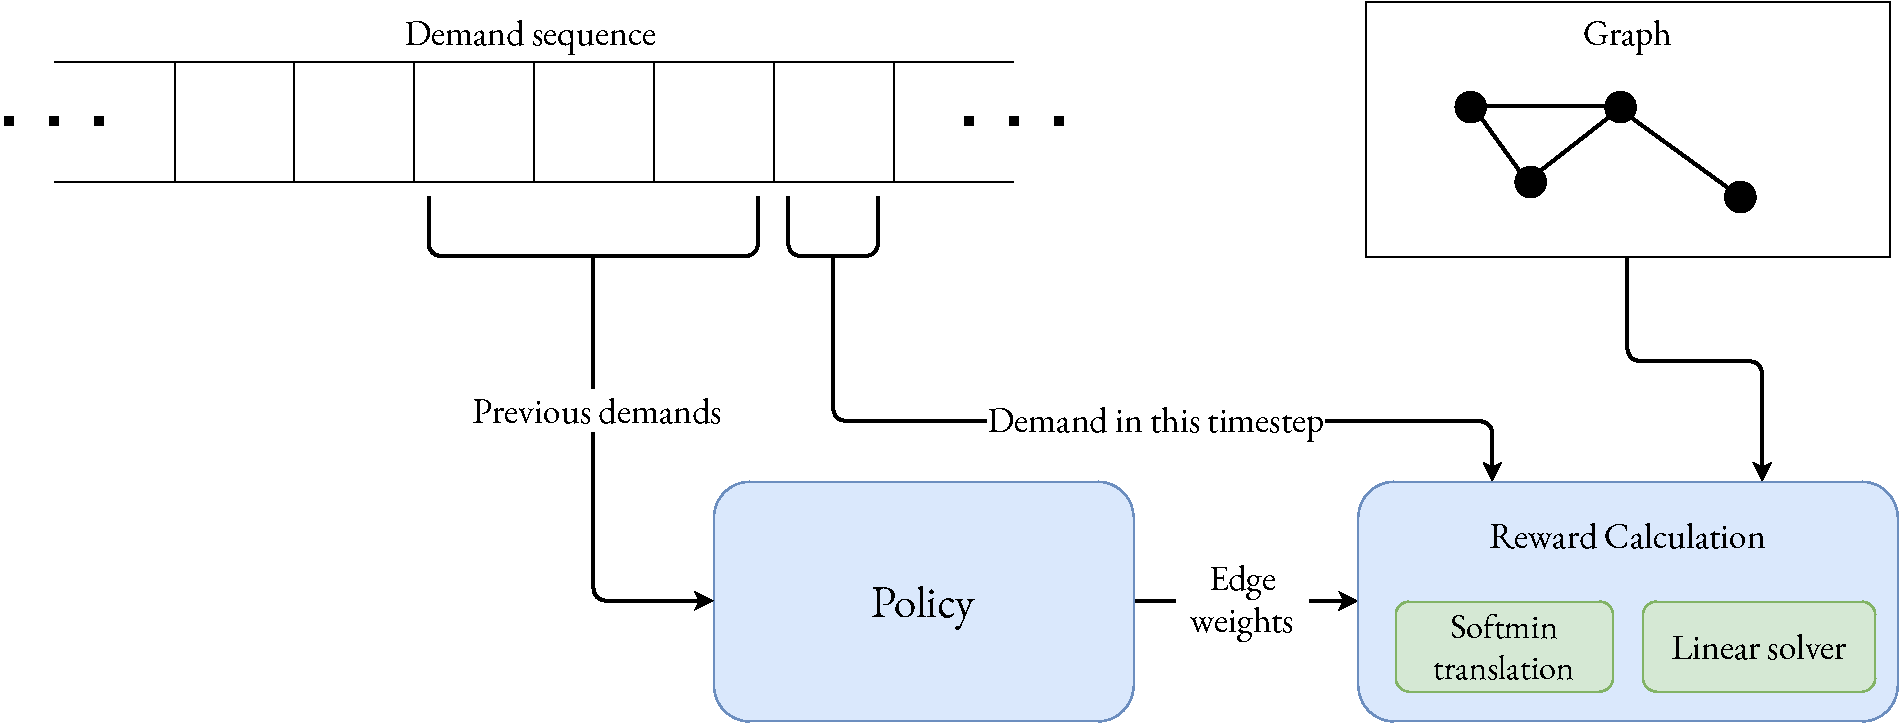
\includegraphics[width=\textwidth]{figures/environment.pdf}
  \caption{Environment dataflow in a single timestep. Top left is the generated demand sequence, and top right is the graph we are outing over. We can see that the previous $n$ demands (here 3) are given to the policy while the reward is calculated using the new demand for this timestep.}
  \label{fig:environment}
\end{figure}

\subsection{Reward calculation}
As the optimal routing that can be achieved on a given graph varies for different demand matrices, the reward cannot simply be derived from the calculation of the maximum link utilisation. Fortunately, as described in section~\ref{section:multicommodity} we know that an optimal routing does exist and it can be found in polynomial time with \ac{lp}. To do this we solve the problem using the standard \ac{lp} formulation, minimising the utility function given in equation~\ref{equation:utility}. Therefore, the environment implements a linear solver for the optimal routing to calculate the optimal link utilisation\footnote{The solver is implemented on top of Google OR-Tools\cite{ortools}}. Then, the reward is derived by comparing the routing produced by the \ac{rl} agent to the calculated optimal routing. The original work used equation~\ref{equation:reward_old} where $U_{max}$ is the maximum link utilisation. However, this reward does not well represent the increased difficulty in improvement the closer the routing is to the optimal and so leads to learning converging too early. To solve this problem we instead used equation~\ref{equation:reward_new} which gives smaller increases in the ratio closer to the optimal congestion a higher relative reward.

\begin{align}
  \begin{split}
    \label{equation:reward_old}
    \mathrm{reward} = -\frac{U_{max_{agent}}}{U_{max_{optimal}}}
  \end{split}\\
  \begin{split}
    \label{equation:reward_new}
    \mathrm{reward} = e^{\frac{U_{max_{optimal}}}{U_{max_{agent}}}}
  \end{split}
\end{align}


\subsection{Observations}
In the original ``Learning to route with Deep RL'' paper, an observation was a history of traffic demands, which was presented as a list of traffic matrices which was then flattened for input to the \ac{mlp}. However, this works aims to make the solution generalisable over graphs of different shapes using \acp{gnn}. As \acp{gnn} work on graphs, it is possible to vary both the number of vertices and edges that are input to a \ac{gnn} (something not possible with an \ac{mlp}). However, this previous way of managing demands as observations would no longer work. The reason for this is that a sensible way to input the demands to the \ac{gnn} would be to place the demands associated with each vertex on that vertex as vertex attributes. The issue here is that the number of demands a vertex has scales with the number of nodes in the graph. Therefore the size of node attributes in the \ac{gnn} would have to grow as more vertices are added which is unfortunately not possible within the structure.

To solve this issue we had to find a way to associate the demands with the correct nodes in a way that would still allow the agent to learn but would require a constant amount of space per vertex as the graph grows. The solution used to this problem was summing for each vertex the total outgoing flow and incoming flow meaning that the observation size is now $O(|V|)$ as opposed to $O(|V|^2)$ and so can be used with a \ac{gnn}.

One other important addition to make this new structure work was normalising the inputs as otherwise the more vertices in a graph, the higher the totals for each vertex will on average be which is unwanted behaviour.

\subsection{Action space}
Following on from the definitions given in section~\ref{section:routing}, we can see that one valid way for the agent to assign a routing would be to provide splitting ratios for each edge under each flow. However, this would require an output of $|V|\times(|V|-1)\times|E|$ separate values. Unfortunately, this size of action space is too big to learn successfully. If we make some approximating assumptions about the routing (which will no longer allow us to achieve the optimal routing but still allow us to get closer than oblivious strategies) then we can reduce this output size.

A first method to reduce the action space size is to ignore the source of any packets, forming a destination-only routing. This reduces the size to $|V|\times|E|$. However, this is still to large so instead we had to create a method of deriving routing strategies from setting weights of edges, creating an action space with only $|E|$ values. This was finally small enough to achieve good results. The next section describes how the routing strategy works.

\section{Softmin routing}
The paper ``Learning to route with Deep RL''\cite{valadarsky2017learning} also ran into the same issues of action space size and so created a method of deriving a routing strategy from edge weights which they called \emph{softmin routing}. As part of our research we attempted to use the same solution specified but found some issues and therefore had to modify it significantly. It is this modified softmin routing that we will present below.

Softmin routing is a way of deriving the splitting ratios on each edge from each vertex, per flow, given weights that have been set on each edge. These values are calculated using algorithm~\ref{algorithm:softmin} which we shall now describe. We calculate the ratios per flow where a flow is a source destination pair, $(s,t)$. For each vertex we calculate its distance to the destination vertex (along its shortest path using the weighted edges). Then, for each vertex we add the weight of each outgoing edge to the distance of the neighbour at the end of that edge. Using the softmin function given in equation~\ref{equation:softmin} with these summed numbers as input, we are returned splitting ratios to use on these edges for routing under this particular flow. This process is then repeated for all vertices and all flows.

\begin{equation}
  \label{equation:softmin}
  \operatorname{softmin}(\bm{x}) = \left(\frac{e^{-\gamma x_i}}{\sum_{j}{e^{-\gamma x_j}}}\right)_i
\end{equation}

One will notice from this description that the routing derived from such a scheme does have a potential flaw. Although it follows all the rules specified for a routing in section~\ref{section:routing} (no traffic is lost and sources send the required demand which is all absorbed by the destination) there is nothing to stop routing loops occurring. An example of such a situation can be seen in figure~\ref{fig:bad_route}. This is undesirable for two reasons. The first is that it wastes capacity as it means traffic traces the same route more than once, and the second is that it increases latency (this is bad but not under measurement here so does not impact our goals). To achieve good results we therefore have to break routing loops.

\begin{figure}
    \centering
    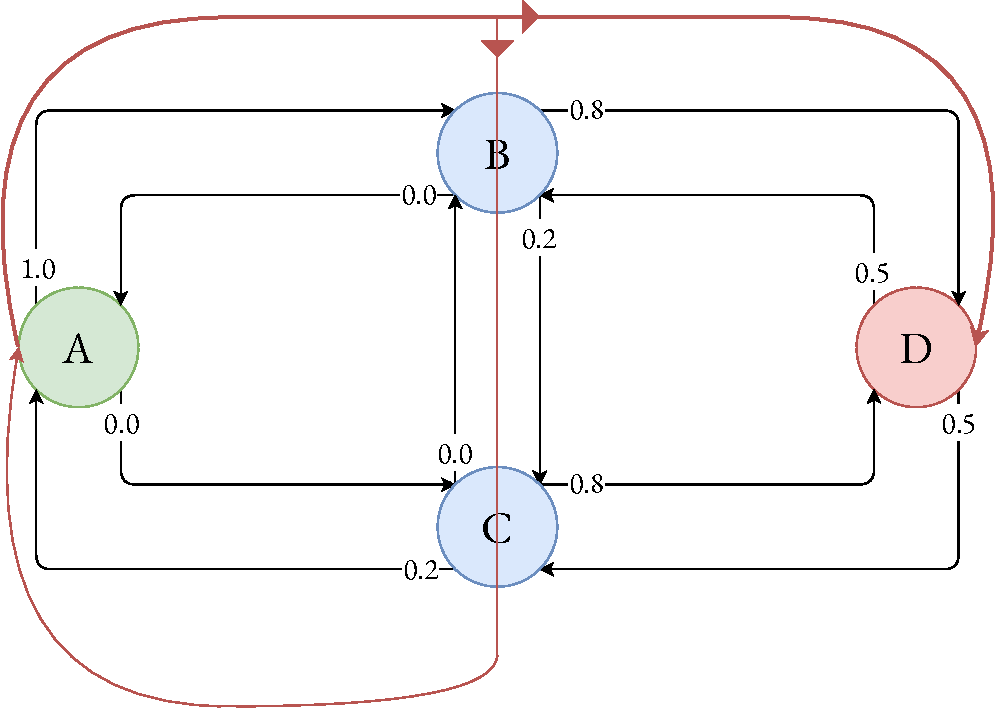
\includegraphics[width=0.8\textwidth]{figures/bad_route.pdf}
    \caption{An example of a bad routing created by the softmin routing strategy. A loop between nodes A, B, and C causes excess link utilisation and increased latency. The circles are vertices with A being the flow source and D the flow destination. The black lines are edges with the numbers signifying their splitting ratios. The red line is the flow induced by this particular routing.}
    \label{fig:bad_route}
\end{figure}

\begin{algorithm}[t]
\small
\begin{algorithmic}
\Function{SoftminRouting}{$G$, $\bm{w}$, $\gamma$}
  \For{$(s, t) \in flows$}
    \State $G \gets \operatorname{PruneGraph}(G, (s, t), \bm{w})$
    \Comment{Convert to a DAG for the source-sink pair}
    \For{$v \in V$}
      \State $d[i] \gets \operatorname{ShortestPath}(i, t)$
      \Comment{Find the distance of each vertex to the sink}
    \EndFor
    \For{$v \in V$}
      \State $out\_edges \gets \operatorname{GetOutEdges}(v)$
      \State $out\_weights \gets \{w[(u, v)] + d[v] | (u, v) \in out\_edges\}$
      \State\Comment{Edge length $+$ neighbour's distance}
      \State $softmin\_weights \gets \operatorname{Softmin}(out\_weights, \gamma)$
      \For{$e \in out\_edges$}
        \State $splitting\_ratios[e] \gets softmin\_weights[e]$
      \EndFor
    \EndFor
  \EndFor
  \State \textbf{return} $splitting\_ratios$
\EndFunction
\end{algorithmic}
\caption{Softmin routing algorithm: the steps taken to convert the learned edge weights given by the \ac{rl} agent into a fully-defined routing strategy.}
\label{algorithm:softmin}
\end{algorithm}

\subsection{Multipath DAG}
The breaking of loops is a problem faced often in routing. In many protocols such as shortest-path based protocols it is not usually an issue as the shortest path by definition cannot contain any cycles but this is not always true as distance vector protocols can run into issues when the network state has not yet converged. It would be easy to remove all loops between source and destination by only keeping the shortest path. However, this does not help with load-balancing and so is not a useful strategy here. What we aim to do is take advantage of multipath with our routings so the longer paths need to remain in the network.

An approach to this problem is looking into ways to convert the graph to a \ac{dag} for each flow where the source and destination become source and sink. Similar work to this is in the use of \ac{dodag} in the \ac{rlp}\cite{rfc6550}. There has been research in the space of constructing \acp{dodag} for multipath applications such as work by Iova et al.\cite{iova2015using} however, being for \ac{rlp}, this focussed on energy minimisation amongst other things.
Therefore, we had to devise a new algorithm to efficiently retain as many paths from destination to source as possible whilst avoiding loops. One attempt was to use a weighted \ac{bfs} from the sink to create a partial ordering on the graph and then only retaining edges that take us closer to the source. However, this still leads to the loss off too many usable links.

The final strategy we devised is shown in algorithm~\ref{algorithm:pruning}. The input to the algorithm is the graph with edges weighted by the agent. We begin by running Dijkstra's algorithm from the source, recording for each node it's parent (in the case of the sink, multiple parents) and any locations where the frontier hits an already explored vertex, called \emph{frontier meets}. Then we trace back from the sink to source, following parent links, and marking any vertex we pass through as \emph{on path}. At this point we have only recorded any shortest paths. Therefore, for every \emph{frontier meet} we find the distance to sink of the first ancestor from each side of the edge to the sink. We then update all the parent information and \emph{on path} information for these vertices so that it becomes a valid path from the more distant ancestor to the closer ancestor. Finally, we remove all edges between nodes that are not \emph{on path} and all edges that are \emph{on path} but where the head of the edge is at the parent.

\begin{algorithm}[t]
\small
\begin{algorithmic}
\Function{PruneGraph}{$(V, E, W), (s,t)$}
  \State $queue \gets [(0, s, [])]$
  \Comment{Queue element is: (distance, vertex, parents)}
  \While{$|queue| \not= 0$}
    \Comment{Run Dijkstra's algorithm}
    \State $(d, v, \bm{p}) \gets \operatorname{pop}(queue)$
    \State $parents[v] \gets \bm{p}$
    \For{$u \in \operatorname{neighbours}(E, v) - \bm{p}$}
      \If{$u = t$}
        \Comment{Stop when reach sink}
        \State $\operatorname{append}(parents[t], v)$
      \ElsIf{$u \in explored$}
        \Comment{Record when see already explored node}
        \State $\operatorname{append}(frontier\_meets, (v, u))$
      \Else
        \State $\operatorname{push}(queue, (d + W(u,v), u, [v]))$
      \EndIf
    \EndFor
    \State $\operatorname{append}(explored, v)$
  \EndWhile

  \State $queue \gets [t]$
  \While{$|queue| \not= 0$}
  \Comment{BFS to mark vertices on path source to sink}
    \State $v \gets \operatorname{pop}(queue)$
    \State $\operatorname{append}(on\_path, v)$
    \For{$p \in parents[v]$}
      \State $d[p] \gets d[v] + G[p][v]$
    \EndFor
  \EndWhile

  \For{$(u,v) \in frontier\_meets$}
    \Comment{Assign paths at frontier collisions}
    \State $a \gets \operatorname{ancestor}(E, on\_path, u)$
    \State $b \gets \operatorname{ancestor}(E, on\_path, v)$
    \If{$d[a] = d[b]$}
      \State \textbf{continue}
    \EndIf
    \State $\operatorname{ConnectPath}(a, u, v, b)$
    \Comment{Update parent pointers for new path}
  \EndFor

  \For{$(u,v) \in E$}
    \Comment{Remove edges not leading to sink}
    \If $u \notin on\_path \wedge v \notin on\_path \wedge u \notin parents[v]$
      \State $E \gets E - \{(u, v)\}$
    \EndIf
  \EndFor
  \State \textbf{return} $(V, E)$
\EndFunction
\end{algorithmic}
\caption{\ac{dag} conversion algorithm retaining high path count from source to sink}
\label{algorithm:pruning}
\end{algorithm}

\section{Traffic demand sequences}
\label{section:demands}
We are using \ac{rl} to approach this problem and the input to the agent is a history of previous demand matrices. The reason for this is that we have made the assumption that the sequence if \acp{dm} will have some sort of regularity which we can exploit to predict a routing strategy for the next timestep that is better than the optimal oblivious routing. Therefore, the demand sequences used for training such an agent must be built using some form of regularity. We try two different types of regularity heavily inspired by those selected by Valadarsky\cite{valadarsky2017learning}.

The first kind of regularity is \emph{cyclical}. Here we generate a cycle of demand matrices and the sequence is simply some number of repetitions of this cycle. The second kind is and \emph{averaging} sequence which is generated by taking a sequence of demand matrices and averaging over the last $n$ when outputting the next demand. These scenarios make sense as temporal regularity is often seen in large networks such as those of \acp{isp}\cite{fortz2002optimizing}.

The demands used to generate the sequences also come in two types. The first is the \emph{bimodal}\cite{medina2002traffic} demand where demands between pairs of nodes are drawn randomly from one of two normal distributions with different means to simulate standard network traffic with occasional elephant flows. The other is a \emph{gravity} demand\cite{roughan2002experience}. This is generated in a deterministic manner taking into account the structure of the network. Effectively we approximate the ingoing flow and outgoing flow to each node from the capacities of their edges. As this demand matrix is deterministic, to add variance allowing us to build sequences of different demands we employ a technique called \emph{sparsification} whereby we stochastically remove demands between some nodes when building the sequence.

The formal definitions for the demand matrix sequences are as follows:
\begin{itemize}
  \item Bimodal DM (parameters given by example values):\\
    $D_{ij} = p$ if $s > 0.8$ else $q$ where $p \sim \mathcal{N}(400, 100), q \sim \mathcal{N}(800, 100), s \sim \mathcal{U}(0,1)$.
  \item Gravity DM:\\
    $D_{ij} = \sum_{(u, v) \in E,\; u = i }{c(u,v)} \times \sum_{(u, v) \in E,\; v = j }{c(u, v)}$ where $c(u,v)$ is the capacity of the edge $(u,v)$.
  \item Cyclical sequence:\\
    $\bm{x} = \left\{ D_{i \mod q} \right\}_{i}$ where $D$ is a sequence of $q$ DMs.
  \item Averaging sequence:\\
    $\bm{x} = \left\{\left(\sum_{j=i-q}^{i}{D_{j \mod q}}\right) / q \right\}_{i}$ where $D$ is a sequence of $q$ DMs.
  \item Sparsification:\\
    $\operatorname{sparsify}(D, p)_{ij} = 0$ if $s > p$ else $D_{ij}$ where $s \sim \mathcal{U}(0,1)$
\end{itemize}

\section{Training graphs}
For training and evaluation purposes it was important that the graphs trained on should be representative of real-world networks. It was thought that maybe graphs from this set could be generated. However, it is difficult to define the set of graphs akin to real-world \ac{as} networks. Fortunately, there is an open dataset, ``The Internet Topology Zoo''\cite{6027859} which contains a plethora of real-world networks, enough for both training and evaluation so it was decided to use this instead.
